\documentclass{beamer}
\usepackage[utf8]{inputenc}

\usetheme{Madrid}
\usecolortheme{default}
\usepackage{amsmath,amssymb,amsfonts,amsthm}
\usepackage{txfonts}
\usepackage{tkz-euclide}
\usepackage{listings}
\usepackage{adjustbox}
\usepackage{array}
\usepackage{tabularx}
\usepackage{gvv}
\usepackage{lmodern}
\usepackage{circuitikz}
\usepackage{tikz}
\usepackage{graphicx}

\setbeamertemplate{page number in head/foot}[totalframenumber]

\usepackage{tcolorbox}
\tcbuselibrary{minted,breakable,xparse,skins}



\definecolor{bg}{gray}{0.95}
\DeclareTCBListing{mintedbox}{O{}m!O{}}{%
  breakable=true,
  listing engine=minted,
  listing only,
  minted language=#2,
  minted style=default,
  minted options={%
    linenos,
    gobble=0,
    breaklines=true,
    breakafter=,,
    fontsize=\small,
    numbersep=8pt,
    #1},
  boxsep=0pt,
  left skip=0pt,
  right skip=0pt,
  left=25pt,
  right=0pt,
  top=3pt,
  bottom=3pt,
  arc=5pt,
  leftrule=0pt,
  rightrule=0pt,
  bottomrule=2pt,
  toprule=2pt,
  colback=bg,
  colframe=orange!70,
  enhanced,
  overlay={%
    \begin{tcbclipinterior}
    \fill[orange!20!white] (frame.south west) rectangle ([xshift=20pt]frame.north west);
    \end{tcbclipinterior}},
  #3,
}
\lstset{
    language=C,
    basicstyle=\ttfamily\small,
    keywordstyle=\color{blue},
    stringstyle=\color{orange},
    commentstyle=\color{green!60!black},
    numbers=left,
    numberstyle=\tiny\color{gray},
    breaklines=true,
    showstringspaces=false,
}
%------------------------------------------------------------
%This block of code defines the information to appear in the
%Title page
\title %optional
{1.4.19}
\date{August 24, 2025}
%\subtitle{A short story}

\author % (optional)
{Aditya Appana - EE25BTECH11004}



\begin{document}


\frame{\titlepage}
\begin{frame}{Question}
Find the position vector of a point \textbf{R} which divides the line joining two points \textbf{P} and \textbf{Q} whose position vectors are $ \hat{i} + 2\hat{j} - \hat{k}$ and $-\hat{i} + \hat{j} + \hat{k} $ respectively in the ratio \textbf{2:1}.
\begin{enumerate}[label=(\alph*)]
    \item externally
    \item internally   
\end{enumerate}

\end{frame}
\begin{frame}{allowframebreaks}
\frametitle{Given Information}

    \centering
    
    \label{tab:parameters}
    
    
    Given vector \mathbf{P} is: \begin{align}
    \myvec{ 1 \\ 2\\ -1}
    \end{align}
    

    Given vector \mathbf{Q} is: \begin{align}\myvec{ -1 \\ 1 \\ 1 }\end{align}
    \label{0.2}

   
\end{frame}


\begin{frame}{Continued}
Let the point which divides $\mathbf{PQ}$ internally be $\mathbf{R}$. \\

Let the point which divides $\mathbf{PQ}$ externally be $\mathbf{S}$. \\

\end{frame}

\begin{frame}{allowframebreaks}
\frametitle{Required Formulae}

    The formula to calculate the coordinates of the point which divides a line segment internally in the ratio m:n is 



\begin{align}
    \mathbf{R}=\frac{\frac{m}{n}\mathbf{P}+\mathbf{Q}}{\frac{m}{n}+1}
\end{align}

and to calculate the coordinates of the point which divides a line segment externally in the ratio m:n is 

\begin{align}
    \mathbf{S}=\frac{\frac{m}{n}\mathbf{P}-\mathbf{Q}}{\frac{m}{n}-1}
\end{align}


\end{frame}


\begin{frame}

\frametitle{Solution}

    Substituting $P\myvec{ 1 \\ 2\\ -1}$ and $Q\myvec{ -1 \\ 1\\ 1}$ in the first formula, we get \vspace{0.5cm}

\begin{align}
    \mathbf{R}=\frac{2\myvec{ 1 \\ 2\\ -1}+\myvec{ -1 \\ 1\\ 1}}{\frac{2}{1}+1} = \frac{\myvec{ 2-1 \\ 4+1\\ -2+1}}{3} = \myvec{ 1/3\\ 5/3\\ -1/3}
\end{align}


\end{frame}


\begin{frame}


\frametitle{Solution}
Substituting $P\myvec{ 1 \\ 2\\ -1}$ and $Q\myvec{ -1 \\ 1\\ 1}$ in the second formula, we get  \vspace{0.5cm}

\begin{align}
    \mathbf{S}=\frac{2\myvec{ 1 \\ 2\\ -1}-\myvec{ -1 \\ 1\\ 1}}{\frac{2}{1}-1} = \frac{\myvec{ 2-(-1) \\ 4-1\\ -2-1}}{1} = \myvec{ 3\\ 3\\ -3}
\end{align}
\end{frame}




\begin{frame}[fragile]
    \frametitle{Python Code}
    \begin{lstlisting}
import sys

import numpy as np

import numpy.linalg as LA
import matplotlib.pyplot as plt

P = np.array([1,2,-1]).reshape(-1,1)
#Defining vector P from the given information

Q = np.array([-1,1,1]).reshape(-1,1) 
#Defining vector Q from the given information

ratio = 2
#Defining the ratio as given in the question

    \end{lstlisting}
\end{frame}

\begin{frame}[fragile]
    \frametitle{Python Code}

    \begin{lstlisting}
R = (ratio*Q + P) / (ratio + 1)
#Calculating vector R with the first formula

S = (ratio*Q - P) / (ratio - 1)
#Calculating vector S with the second formula

    \end{lstlisting}
\end{frame}

\begin{frame}[fragile]
    \frametitle{Python Code}

    \begin{lstlisting}
x_PQ = np.block([P,Q,R,S])
fig = plt.figure(figsize=(8, 6))
ax = fig.add_subplot(111, projection='3d')

ax.plot(x_PQ[0,:],x_PQ[1,:], x_PQ[2,:],label='$BC$')
#Plotting all lines

all_coords = np.block([P, Q, R, S])  # Stack A, B, C vertically
ax.scatter(all_coords[0, :],all_coords[1, :],all_coords[2, :])
vert_labels = ['P', 'Q', 'R', 'S']

for i, txt in enumerate(vert_labels):
    ax.text(all_coords[0, i], all_coords[1, i], all_coords[2, i], f'{txt}\n({all_coords[0, i]:.0f}, {all_coords[1, i]:.0f}, {all_coords[2, i]:.0f})',
             fontsize=12, ha='center', va='bottom')

#Plotting the points and labelling them

\end{lstlisting}
\end{frame}

\begin{frame}[fragile]
    \frametitle{Python Code}

    \begin{lstlisting}

ax.spines['top'].set_color('none')
ax.spines['left'].set_position('zero')
ax.spines['right'].set_color('none')
ax.spines['bottom'].set_position('zero')

plt.grid() # minor
plt.axis('equal')

plt.show()

    \end{lstlisting}
\end{frame}

\begin{frame}{Plot}
    \begin{center}
        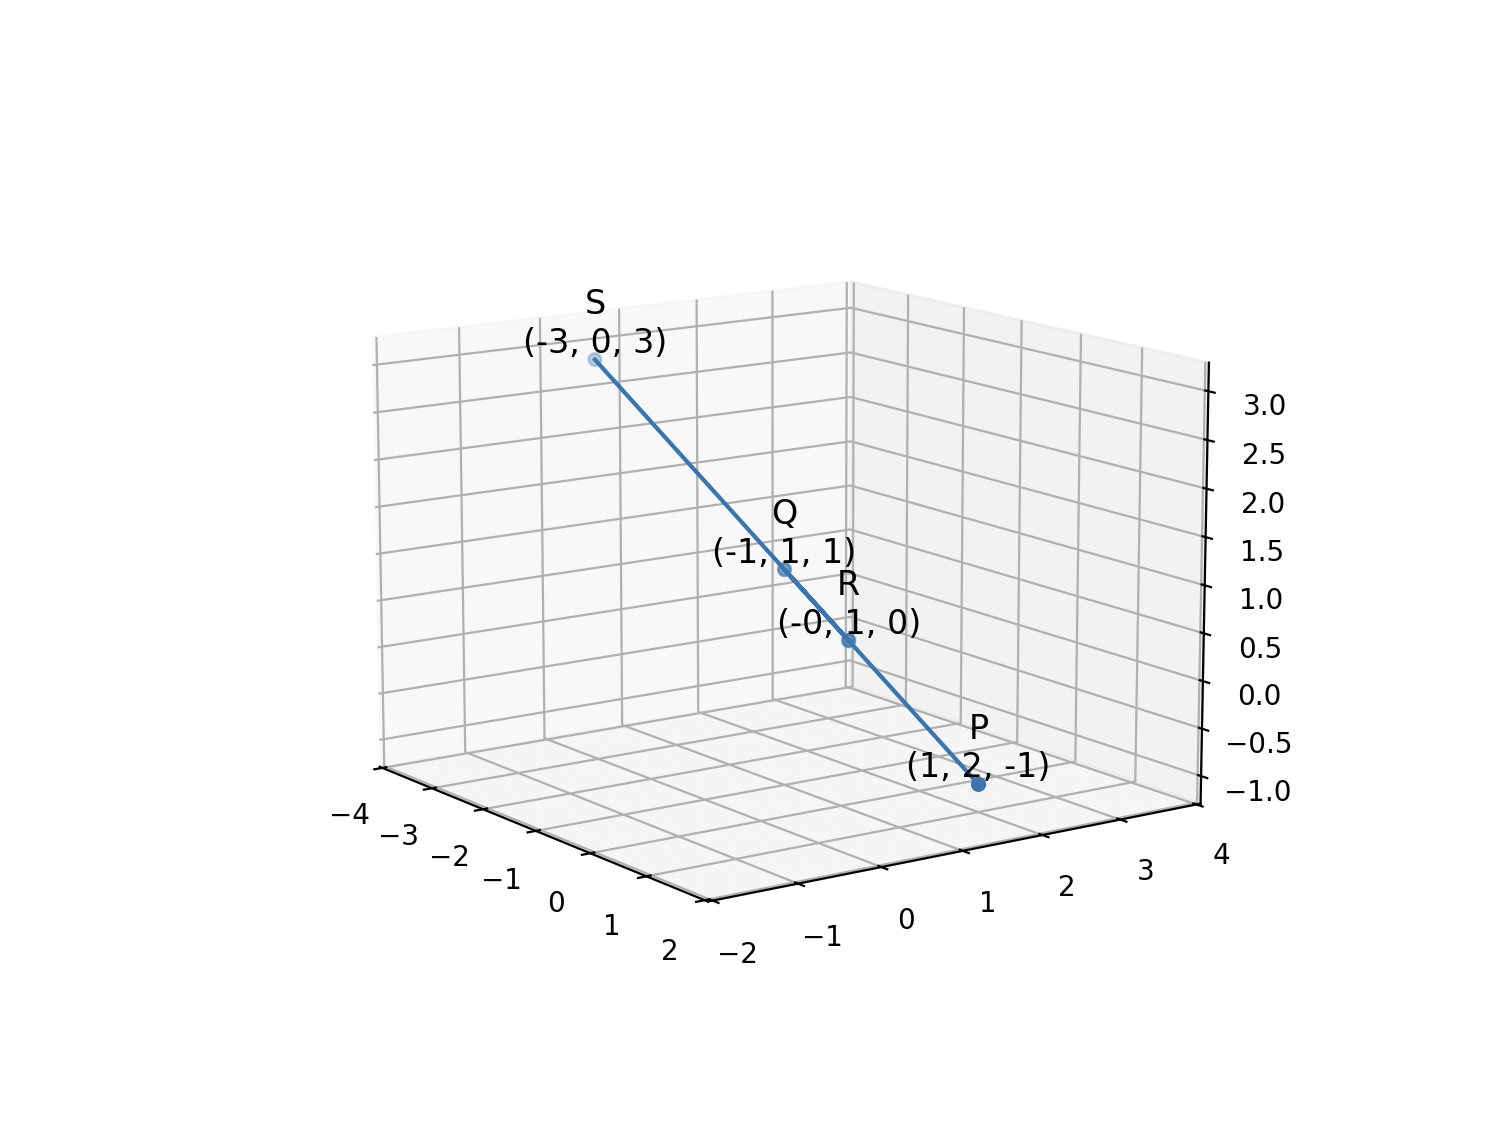
\includegraphics[width=\linewidth]{Figs/Figure_1.png}
    \end{center}
\end{frame}





\end{document}